\documentclass[a4paper,14pt]{extarticle} %extrarticle
\usepackage[T2A]{fontenc}
\usepackage[utf8]{inputenc}
\usepackage[russian,english]{babel}
\usepackage[pdftex,unicode]{hyperref}
%\usepackage{pscyr}
\usepackage{cmap}
\ifx\pdfoutput\undefined
\usepackage{graphicx}
\else
\usepackage[pdftex]{graphicx}
\fi

\usepackage{amstext}
\usepackage{amssymb}
\usepackage{lscape}
\usepackage{makecell}
\usepackage{multirow}
\usepackage{multicol}
\usepackage{ulem}
\usepackage{indentfirst}
\setcounter{tocdepth}{3}
\usepackage{url} % для url'ов

% выставляем параметры страниц
\usepackage{geometry}
\geometry{verbose,a4paper,tmargin=2cm,bmargin=2cm,lmargin=2.5cm,rmargin=1cm}

% меняем шрифт на Times New Roman
%\usepackage{times}
%\renewcommand{\rmdefault}{ftm}
%\renewcommand\theadfont{\normalsize}

% меняем шрифты
%\renewcommand\large{\@setfontsize\large{15.5}{17}}
%\renewcommand\Large{\@setfontsize\Large{16.5}{19}}


\linespread{1.3} % 1,5
\graphicspath{{../images/}}

\begin{document} % начало документа
\sloppy

\begin{titlepage} % начало титульной страницы

\thispagestyle{empty}

\begin{center}
	\small{
    	\textbf {
        	Министерство образования и науки Российской Федерации \\
            Государственное образовательное учреждение высшего профессионального образования \\
            ДАЛЬНЕВОСТОЧНЫЙ ГОСУДАРСТВЕННЫЙ УНИВЕРСИТЕТ \\
            \smallskip \hrule height 2pt \smallskip \hrule \smallskip
            ИНСТИТУТ МАТЕМАТИКИ И КОМПЬЮТЕРНЫХ НАУК \\
            Кафедра информатики \\
    \vspace{2cm}
    ОТЧЕТ \\
        }
    о прохождении преддипломной практики \\
    }
    \vspace{4cm}

\end{center}
\small{
\begin{multicols}{2}
    \verb""\\
    \bigskip

    Отчет защищен: \\
    с оценкой \\
    \rule{5cm}{0.5pt} \\
    \rule{3cm}{0.5pt} М.А.Гузев \\
    <<\rule{1cm}{0.5pt}>> марта 2010г. \\

    \smallskip

    Регистрационный № \rule{1cm}{0.5pt} \\
    \rule{5cm}{0.5pt} \\

    \smallskip

    <<\rule{1cm}{0.5pt}>> марта 2010г. \\

    \bigskip

    Выполнил студент гр. 258 \\
    \rule{4cm}{0.5pt} А.Е.Антонов \\
    Руководитель практики \\
    заведующий лабораторией машинной графики ИАПУ ДВО РАН, д.т.н.\\
    \rule{4cm}{0.5pt} В.А.Бобков \\

    \bigskip

    Практика пройдена в срок \\
    с <<\rule{1cm}{0.5pt}>> декабря 2009г. \\
    по <<\rule{1cm}{0.5pt}>> марта 2010г. \\
    на предприятии \\
    ДВГУ, Кафедра информатики \\

\end{multicols}

\vfill

\begin{center}
    г. Владивосток\\
    2010
\end{center}
}
\end{titlepage} % конец титульной страницы

\setcounter{page}{2}
% меняем оформление оглавления
\begin{center}
\renewcommand{\contentsname}{Оглавление}
\tableofcontents % содержание
\end{center}

\newpage

\section{Введение}

\subsection{Глоссарий}
\textbf{Воксел} -- элемент объёмного изображения, содержащий значение элемента растра в трёхмерном пространстве. Вокселы являются аналогами пикселов для трехмёрного пространства.~\cite{wiki_voxel}

\textbf{Кроссплатформенное программное обеспечение} -- программное обеспечение, работающее более чем на одной аппаратной платформе и/или операционной системе.~\cite{wiki_crossplatfom}

\textbf{ПК} -- персональный компьютер.

\textbf{Реконструкция} -- построение объемной модели реального объекта.

\textbf{Фреймворк} -- в информационных системах структура программной системы; программное обеспечение, облегчающее разработку и объединение разных компонентов большого программного проекта. В его состав могут входить вспомогательные программы, библиотеки кода, язык сценариев и проч.~\cite{wiki_framework}

\subsection{Описание предметной области}
Потребность в реалистичном отображении окружающего мира увеличивает значимость трехмерного (3D) моделирования -- построения компьютерных моделей объектов. 3D модели облегчают планирование, контроль и принятие решений во многих отраслях. Например, если в ходе эксплуатации модели требуется внести коррективы, компьютерный объект позволит это сделать максимально быстро.

Особенно сложной проблемой является создание точных моделей объектов из реального мира.~\cite{komarova_voxel_coloring} Как быстро выяснилось, человеческий глаз очень легко определяет погрешности в синтезированных изображениях хорошо известных ему в повседневной жизни объектов.

Вот несколько примеров объектов, требующих реконструкции:
\begin{enumerate}
\item Здания и строения
\item Предприятия со сложной структурой (нефтегазоперерабатывающие комплексы, химические предприятия и т.д.)
\item Дороги и дорожные объекты (мосты, путепроводы, прилегающая зона)
\item Открытые и закрытые горные разработки
\item Рельефы местности
\end{enumerate}

\subsubsection{Методы построения моделей объектов}
На данный момент существует три основных способа получения модели объекта:
\begin{itemize}
\item Использование активных методов (например, лазерных сканеров, позволяющих с высокой точностью определить расстояние от лазера до поверхности объекта)
\item Вручную с помощью программ трехмерного моделирования (например, Blender, 3D Studio Max)
\item Автоматическая реконструкция объекта по набору изображений и другой известной о нем информации
\end{itemize}

Сканеры -- современное средство измерения, позволяющее производить исполнительную съемку сложных объектов, там, где проходит множество пересечений на различных уровнях. Причем вступать в контакт с самим объектом не требуется. Сканер формирует модель по десяткам тысяч точек, при этом положение каждой из них определяется с точностью от 2--3 мм до 2 см. Наземные сканеры используются для создания моделей зданий, заводов, кварталов и других больших сооружений. Дальность сканера составляет порядка 200 метров, на таком расстоянии он может определять объекты с точностью шага до 0.5 см. Современные сканеры в состоянии сканировать окружающую действительность с поворотом на 360 градусов, что позволяет сканировать сразу несколько зданий. Сшивка отдельных сканов выполняется посредством специальных марок или характерных точек рельефа. Такой метод обеспечивает высокое качество проектирования, приближая его к реальности. Недостатками использования сканера являются высокая стоимость оборудования (от 50 тыс. долл.~\cite{laser_scanner}), необходимость в высококвалифицированных специалистах, способных это оборудование обслуживать, а так же невозможность реконструкции динамических сцен.~\cite{komarova_voxel_coloring}

Второй подход требует больших затрат усилий и времени, что вытекает в высокую стоимость и длительные сроки разработки модели.

В третьем подходе в качестве исходных данных используют только фотографии или последовательности изображений объектов, полученные в естественном освещении, или приближенном к нему (в свете обычных ламп). Такой подход считается наиболее перспективными, так как позволяет строить модели динамических сцен, в которых могут участвовать люди.

\subsection{Неформальная постановка задачи}
Создание кроссплатформенного приложения, использующего для реконструкции объекта алгоритм раскраски вокселей по методу множества гипотез~\cite{multi_hypothesis} и способного задействовать все возможности современного ПК. Из поставленных условий вытекает еще одна задача -- распараллеливание существующего алгоритма.

\subsection{Математические методы}
В качестве базового, для построения модели объекта, используется алгоритм раскраски вокселей по методу множества гипотез~\cite{multi_hypothesis}.

\subsection{Обзор существующих методов решения}

На текущий момент была найдена только одна, находящаяся в открытом доступе, реализация алгоритма раскраски вокселей -- Voxel Coloring Framework~\cite{voxel_coloring_framework}. К её достоинствам можно отнести распространение под академической свободной лицензией~\cite{academic_free_license}. Однако данная реализация обладает следующими недостатками:
\begin{itemize}
\item Работает только в операционной системе семейства MS Windows
\item Для работы необходим пакет Matlab
\item Не использует вычислительные возможности современных графических адаптеров
\end{itemize}

\section{Требования к окружению}

\subsection{Требования к аппаратному обеспечению}
Необходимо наличие в системе устройств с поддержкой стандарта OpenCL~\cite{opencl_standart}. Список поддерживаемых устройств можно найти 
\begin{itemize}
\item для NVIDIA в \cite{opencl_nvidia_support}
\item для ATI в \cite{opencl_ati_support}
\item для S3 в \cite{opencl_s3_support}
\item для IBM в \cite{opencl_ibm_support}
\end{itemize}

\subsection{Требования к программному обеспечению}
Для работы приложения необходимо наличие в системе установленной библиотека Qt версии не ниже 4.6, а так же драйверов для устройств с поддержкой стандарта OpenCL версии 1.0.

\section{Спецификация данных}
\subsection{Формат метафайла}
Метафайл -- файл, используемый для сохранения и последующего восстановления информации о загруженных пользователем изображениях, введенных матрицах внешней и внутренней калибровки, объемлющем основной объект прямоугольнике. Этот файл записан в текстовом формате. Файл имеет следующую структуру:
\begin{itemize}
\item В первой строке находится беззнаковое целое число, обозначающее количество изображений, информация о которых записана в файле.
\item Далее идет три строки, содержащие по три элемента, разделенных пробелами. Каждый элемент -- число с плавающей точкой. Вместе они описывают матрицу внутренней калибровки камеры.
\item Далее идет информация об изображениях:
	\begin{itemize}
		\item имя файла с изображением, записанное в формате, совместимом с типом QString (см.~\cite{qt_qstring})
		\item прямоугольник, объемлющий основной объект, записанный в формате, совместимом с типом QRectF (см.~\cite{qt_qrectf})
		\item матрица внешней калибровки камеры для данного изображения, записанная в три строки по три числа с плавающей точкой в каждой.
	\end{itemize}
Количество таких блоков должно быть равным числу, записанном в первой строке файла.
\end{itemize}


\section{Функциональные требования}
Система должна позволять пользователю:
\begin{itemize}
\item загружать изображения
\item выделять основной объект
\item вводить матрицу внешней калибровки камеры для каждого изображения
\item вводить матрицу внутренней калибровки камеры
\item запускать выполнение алгоритма построения вокселной модели, на основе загруженных изображений
\item просматривать полученную воксельную модель объекта
\item сохранять и загружать метафайл
\item сохранять построенную воксельную модель
\item загружать для просмотра воксельную модель
\end{itemize}


\section{Требования к интерфейсу}
Система должна иметь приложение с графическим интерфейсом пользователя. Графический интерфейс должен предоставлять всю функциональность библиотеки.

\section{Проект}
\subsection{Средства реализации}
Для реализации приложения был выбран язык программирования C++, т.к. он очень распространен, что упрощает последующую поддержку приложения. К тому же, программы, написанные на этом языке, могут быть скомпилированы для очень большого количества платформ.

Для упрощения переноса приложения на другие платформы, был использован кроссплатформенный инструментарий разработки ПО под названием Qt. Он так же включает в себя инструментарий, необходимый для разработки кроссплатформенных приложений с графическим интерфейсом пользователя. Выбор этого инструментария позволяет уменьшить усилия, требуемые для реализации новой и поддержки имеющейся функциональности.

Для того, чтобы приложение могло задействовать как можно больше доступных ресурсов современных ПК, было решено использовать фреймворк OpenCL. Это позволит приложению задействовать ресурсы всех процессоров в многопроцессорных системах, а так же ресурсы современных видеокарт.
Для взаимодействия с OpenCL используется экспериментальный биндинг для языка C++~\cite{opencl_bindings}, который предоставляет ООП-интерфейс для доступа к OpenCL.

\section{Модули и алгоритмы}
Составляющими элементами системы являются библиотека covc и набор приложений:
\begin{itemize}
\item oclc
\item qcovc
\item ocl\_volume\_render
\end{itemize}


\subsection{Библиотека covc}
Библиотека covc содержит реализацию алгоритма раскраски вокселей методом множества гипотез.

\subsubsection{Программный интерфейс библиотеки}
Программный интерфейс библиотеки состоит из следующих функций:
\begin{itemize}
\item \textit{add\_image} -- добавление нового изображения
\item \textit{build\_voxel\_model} -- запуск алгоритма
\item \textit{get\_voxel\_model} -- получение результирующей вокселной модели
\item \textit{prepare} -- инициализация библиотеки
\item \textit{set\_camera\_calibration\_matrix} -- ввод матрицы внутренней калибровки камеры
\item \textit{set\_number\_of\_images} -- ввод количества изображений
\item \textit{set\_resulting\_voxel\_cube\_dimensions} -- ввод размерностей результирующей вокселной модели
\end{itemize}

\subsection{Алгоритм раскраски вокселей}
Все операции в процессе реконструкции производятся над вокселами, которые уникальны для трехмерной модели объекта, а не над пикселями, которых несколько для одного воксела. Поэтому не нужно специально вычислять точки соответствия и по ним вычислять карту глубины.

В реализованном алгоритме четыре этапа:
\begin{enumerate}
\item Вычисление объемлющего трехмерного куба объекта
\item Инициализация вокселей, назначение каждому вокселю гипотез
\item Первоначальная отбраковка ложных гипотез
\item Дальнейшая проверка гипотез на соответствие по всем изображениям и  удаление ложных гипотез
\end{enumerate}

\subsubsection{Вычисление объемлющего трехмерного куба объекта}
В начале работы программы можно ограничить пространство, в котором располагается реконструируемый объект. Для этого пользователь на изображениях выделяет рамкой объект. Затем, используя калибровочные данные, вычисляется объемлющий объект объем (bounding volume). Для его расчета на каждом отмеченном рамкой изображении считается двумерный центр этой рамки. Если рамка не задана, то в используется двумерный центр изображения. По всем полученным двумерным центрам и матрицам внешней калибровки считается трехмерный центр всех рамок, отмеченных пользователем, и изображений. Впоследствии этот центр будет центром полученного объемлющего куба.

Трехмерные координаты камеры $[x;y;z]^T$ можно найти так:

\begin{center}
	$[x;y;z;w]^T = C^{-1}*[0;0;0;1]^T$ , где
\end{center}
$C$ - матрица внешней калибровки изображения, полученного с этой камеры.

Каждое изображение относительно своей камеры находится на расстоянии~1. Считаем трехмерные координаты $[X_{3D};Y_{3D};Z_{3D}]^T$ углов отмеченных рамок и изображений следующим образом:

\begin{center}
	$K^{-1}*[x;y;1]^T = [X;Y;Z]^T$ \\
	$[X_{3D};Y_{3D};Z_{3D}]^T = C^{-1}*[X;Y;Z]^T$ , где
\end{center}
$C$ - матрица внешней калибровки изображения;\\
$K$ - матрица внутренней калибровки камеры;
$[x;y;1]$ - координаты в пикселях угла выделенной рамки или изображения.

На рисунке ниже $OD = 1$; треугольник ${OAD}$ подобен треугольнику ${OBC}$. Требуется вычислить координаты точки $B$, если известны трехмерные координаты $A$, $O$, $C$:

\begin{center}
	$\frac{OB}{OA} = \frac{OC}{OD} = \frac{OC}{1} \Rightarrow OB = OA*OC$ \\
	$B = O + AO*OC$
\end{center}

\begin{figure}[h]
\center
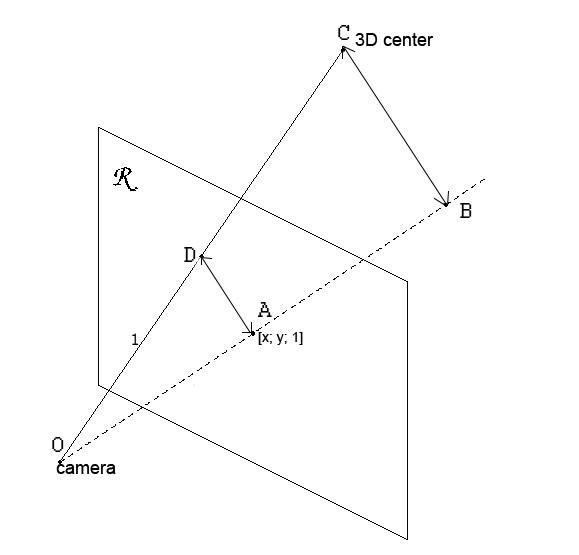
\includegraphics[scale=0.5]{3dcenter}
\caption{Вычисление трехмерных координат точек изображения}
\end{figure}

Таким образом, вычисляем трехмерные координаты всех углов отмеченных пользователем рамок. Далее можем вычислить трехмерную высоту и ширину выделенной рамки для каждого изображения. Считаем максимум среди этих расстояний. Полученное значение будем считать за сторону трехмерного куба, объемлющего объект.

\subsubsection{Инициализация вокселей, назначение каждому вокселю гипотез}
На следующем этапе для каждого изображения составляется матрица проекции:

\begin{center}
	$P = K*I*C$, где
\end{center}
$K$ - матрица внутренней калибровки камеры
$I$ - единичная матрица
$C$ - матрица внешней калибровки изображения.

Проекция воксела на изображение (координаты $x$ и $y$ в пикселях) получается умножением слева матрицы проекции данного изображения на трехмерный центр воксела:

\begin{center}
	$[x;y;z]^T = P*[X_{3D};Y_{3D};Z_{3D};1]^T$ \\
	$x = x/z$ \\
	$y = y/z$
\end{center}

Обходя все вокселы, для каждого воксела составляем гипотезы. Каждая гипотеза – это цвет проекции воксела на изображение в цветовом пространстве RGB. Для увеличения надежности алгоритма каждая компонента цвета гипотезы делится на сумму всех компонент (red + green + blue) этой гипотезы. Итого, для каждого воксела должно быть столько гипотез, сколько изображений во входной последовательности. Но если проекция воксела на изображение -- точка с пиксельными координатами $[x;y]$ -- выходит либо за границы изображения, либо за пределы выделенной пользователем рамки, соответствующая гипотеза считается ложной.

Сначала все вокселы видимые. Если все гипотезы для какого-либо воксела оказались ложными, этот воксел считается невидимым.

\subsubsection{Первоначальная отбраковка ложных гипотез}
Проходя последовательно по всем вокселам, для каждой гипотезы текущего воксела сравниваем ее со всеми остальными гипотезами для этого воксела. Гипотеза(1) считается верной, если найдется другая гипотеза(2) данного воксела, такая, что расстояние между этими гипотезами в цветовом пространстве RGB меньше заданного порога $T$:

\begin{center}
	$\lvert {red(0)} - {red(1)}\rvert + \lvert {green(0)} - {green(1)}\rvert + \lvert {blue(0)} - {blue(1)}\rvert < T$
\end{center}

Получим, что гипотеза ложная только в том случае, когда она не соответствует ни одной другой гипотезе для данного воксела. Так же как и ранее воксел считается невидимым, если все связанные с ним гипотезы ложны.

Далее считается, сколько осталось верных гипотез и изменяется порог $T$:

\begin{center}
	$T_{new} = T/{dim_x*dim_y*dim_z*N}$, где
\end{center}
$T_{new}$ - новое значение порога;\\
$dim_x, dim_y, dim_z$ - размерности результирующей модели по $x,y,z$ соответственно;\\
$N$ - количество изображений во входной последовательности.

Такое изменение порога позволяет более точно в дальнейшем определять ложные гипотезы.

\subsubsection{Дальнейшая проверка гипотез}

Алгоритм построен так, что он учитывает с какой стороны нужно рассматривать объемлющий куб для каждого изображения. Это сделано для того, чтобы правильно устанавливать видимость вокселей с каждого изображения. 

Чтобы найти порядок обхода вокселей для данного изображения, вычисляем расстояния в трехмерных координатах между камерой и всеми восемью углами объемлющего куба. Ближайший угол определяет порядок обхода вокселей: этот угол нужно обойти раньше остальных. 

В соответствующем порядке обходим куб и отбраковываем гипотезы как ранее:   
гипотеза ложная только в том случае, когда она не соответствует ни одной другой гипотезе для данного воксела, то есть:

\begin{center}
	$\lvert {red(i)} - {red(j)}\rvert + \lvert {green(i)} - {green(j)}\rvert + \lvert {blue(i)} - {blue(j)}\rvert > T_{new}$
\end{center}
при фиксированном $i$ для всех $i \neq j$.

Кроме того, для каждого изображения заводятся буфера – матрицы той же размерности, что и сами изображения на которых будут отмечаться видимые вокселы. Первоначально буфера пусты. Рассматривая каждую гипотезу проверяем, занят ли буфер на ее месте. Для этого вычисляем, какому вокселу соответствует эта гипотеза, Проецируем воксел на текущее изображение. Если буфер не занят, то заполняем его в тех  позициях, куда проецируется весь воксел (это может быть несколько пикселей). Если же буфер уже занят, то данный воксел не видим на этом изображении, и его гипотезу можно не рассматривать.    

Так обходятся все изображения в нужном порядке до тех пор, пока хоть одна гипотеза признается ложной. 

В итоге получаем вокселную модель реконструируемого объекта.

\newpage
\subsection{Реализация алгоритма}
Схематически алгоритм изображен на диаграмме ниже.
\begin{figure}[h]
\center
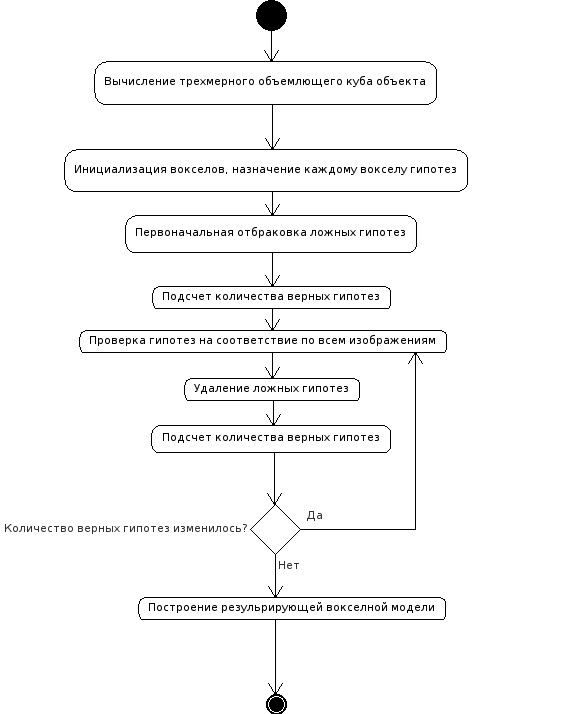
\includegraphics[scale=0.7]{qcovcactivitydiagram}
\caption{Диаграмма активности}
\end{figure}

На этапах <<Инициализация вокселей, назначение каждому вокселу гипотез>>, <<Первоначальная отбраковка ложных гипотез>>, <<Подсчет количества верных гипотез>> и <<Удаление ложных гипотез>> было применено распараллеливание вычислений.

\subsection{Приложение oclc}
Данное приложение является оберткой над компилятором OpenCL C. Оно позволяет проверить на корректность программы, написанные на языке OpenCL C и получить описание допущенных ошибок.

\subsection{Приложение qcovc}
Данное приложение позволяет пользователю, при помощи графического интерфейса, работать с библиотекой.

\subsubsection{Классы приложения}
\begin{itemize}
\item \textit{MainWindow} -- главное окно приложения
\item \textit{ImageInfo} -- информация об изображении
\item \textit{ImagePreview} -- виджет предпросмотра изображений
\item \textit{ImageScene} -- сцена для отображения изображения
\end{itemize}

\subsubsection{Класс MainWindow}
Методы класса:
\begin{itemize}
\item \textit{add\_image} -- добавление нового изображения
\item \textit{load\_metafile} -- загрузка метафайла
\item \textit{save\_metafile} -- сохранение метафайла
\end{itemize}

\subsubsection{Класс ImagePreview}
Методы класса:
\begin{itemize}
\item \textit{add\_image} -- добавление нового изображения в блок предпросмотра
\item \textit{clear} -- очистка блока предпросмотра
\end{itemize}

\subsubsection{Класс ImageScene}
Методы класса:
\begin{itemize}
\item \textit{rectangle\_changed} -- изменяет параметры объемлющего прямоугольника для изображения
\item \textit{set\_rectangle} -- устанавливает объемлющий прямоугольник для отображения
\item \textit{set\_image} -- устанавливает изображение для отображения
\end{itemize}

\subsubsection{Диаграмма классов}
\begin{figure}[h]
\center
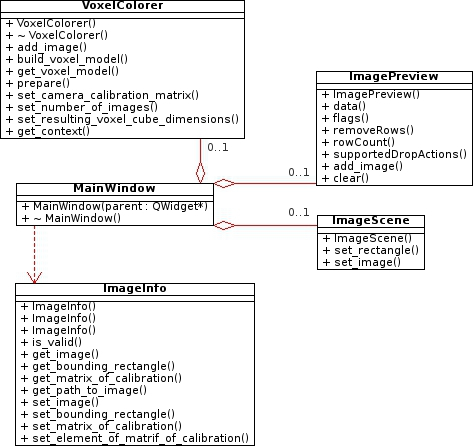
\includegraphics[scale=0.7]{qcovcclassdiagram}
\caption{Диаграмма классов приложения qcovc}
\end{figure}

\subsubsection{Проект интерфейса}
Из меню графического интерфейса пользователя должно быть доступно сохранение и загрузка метафайла, добавление нового изображения, запуск на выполнение алгоритма получения объемной модели объекта. Основное окно должно быть разделено на три части: слева должны находиться блок просмотра миниатюр изображений и блок ввода матрицы внешней калибровки камеры для выбранного изображения. Остальную часть окна должен занимать блок, в который выводится текущее выбранное изображение. Так же в этом блоке должно быть доступно выделение объемлющего прямоугольника.
\begin{figure}[h]
\center
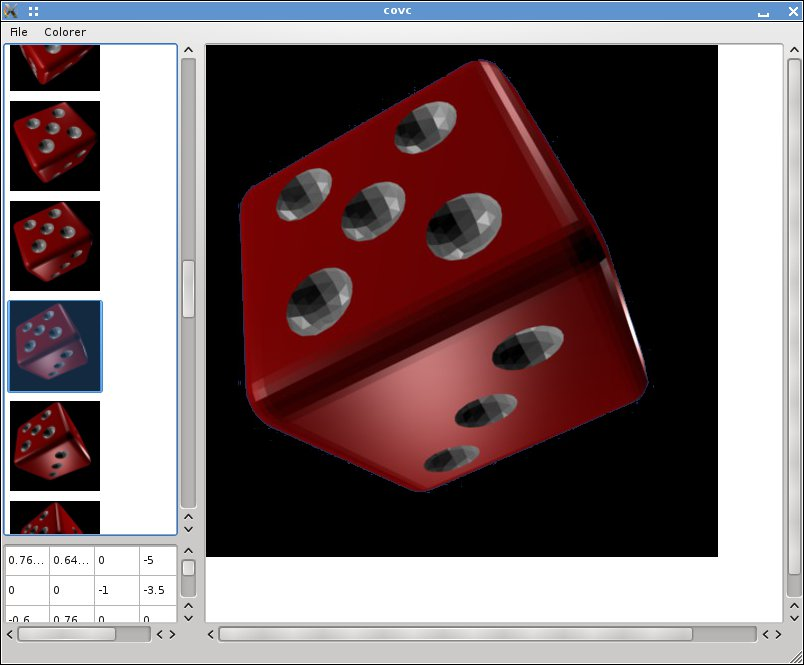
\includegraphics[scale=0.5]{gui}
\caption{Проект интерфейса}
\end{figure}

\newpage
\subsection{Приложение ocl\_volume\_render}
Данное приложение является модифицированной версией программы oclVolumeRender из комплекта NVIDIA GPU Computing SDK~\cite{nvidia_gpu_sdk} и позволяет пользователю просматривать полученную воксельную модель.



\section{Реализация и тестирование}
Объем итогового кода на С++ составляет 17.9 Кб в 12 файлах.\\
Объем автоматически сгенерированного кода (XML) составляет 3 Кб.\\
На текущий момент кодовая база содержит 4,693 строки.


\section*{Заключение}
В настоящий момент сделан набросок интерфейса, реализованы функции добавления изображения, загрузки метафайла, выделения основного объекта, ввода матрицы внешней калибровки камеры. В дальнейшем необходимо реализовать функцию сохранения метафайла, алгоритм построения воксельного объекта на основе изображений и введенных данных и функцию просмотра полученной воксельной модели объекта.



\renewcommand{\refname}{Список литературы}
\begin{thebibliography}{99}

	\bibitem{academic_free_license}
		Academic Free License ("AFL") v. 3.0 [Электронный~ресурс] : электрон.~энциклопедия -- Режим доступа:
		\url{http://www.opensource.org/licenses/academic.php}

	\bibitem{opencl_ati_support}
		ATI, ATI Stream Software Development Kit [Электронный~ресурс]
		 -- Режим доступа:
		\url{http://developer.amd.com/gpu/ATIStreamSDK/Pages/default.aspx#two}
	
	\bibitem{bsd}
		<<Simplified BSD License>> [Электронный~ресурс] : электрон.~энциклопедия -- Режим доступа:
		\url{http://www.opensource.org/licenses/bsd-license.php}
	
	\bibitem{chien}
		Chien C.H., Aggarwal J.K. Identification of 3D Objects from Multiple Silhouettes Using Quadtrees/Octrees // 
		Computer Vision Graphics And Image Processing -- 1986 -- PP. 256-273

	\bibitem{opencl_bindings}
		Experimental C++ Bindings to OpenCL [Электронный~ресурс] -- Режим доступа:
		\url{http://www.khronos.org/registry/cl/}
	
	\bibitem{foxc}
		Fixstars OpenCL Cross Compiler [Электронный~ресурс] -- Режим доступа:
		\url{http://www.fixstars.com/en/foxc/}
		
	\bibitem{opencl_ibm_support}
		IBM, OpenCL Development Kit for Linux on Power [Электронный~ресурс]
		-- Режим доступа:
		\url{http://www.alphaworks.ibm.com/tech/opencl}

	\bibitem{laser_scanner}
		Leica ScanStation 2 3D Laser Scanner [Электронный~ресурс] //
		FLT~Geosystems~website -- Режим доступа:
		\url{http://www.fltgeosystems.com/}

	\bibitem{multi_hypothesis}
		Eisert, P. Multi-Hypothesis, volumetric reconstruction of 3-d objects from multiple calibrated camera views /
		Peter Eisert, Eckehard Steinbach, Bernd Girod //
		ICASSP’99, Phoenix, USA -- march~1999. -- PP. 3509-3512

	\bibitem{opencl_standart}
		Khronos Group, OpenCL [Электронный~ресурс] -- Режим доступа:
		\url{http://www.khronos.org/opencl/}

	\bibitem{voxel_coloring_framework}
		Koen van de Sande, Voxel Coloring Framework [Электронный~ресурс]
		-- Режим~доступа:
		\url{http://voxelcoloring.sourceforge.net/}

	\bibitem{aggarwal}
		Martin W.N., Aggarwal J.K. Volumetric description of objects from multiple views //
		IEEE Transactions on Pattern Analysis and Machine Intelligence. -- 1983

	\bibitem{qt_qrectf}
		Nokia, QRectF [Электронный~ресурс]
		-- Режим доступа:
		\url{http://doc.trolltech.com/4.6/qrectf.html}

	\bibitem{qt_qstring}
		Nokia, QString [Электронный~ресурс]
		-- Режим доступа:
		\url{http://doc.trolltech.com/4.6/qstring.html}

	\bibitem{opencl_nvidia_support}
		NVIDIA, CUDA GPUs [Электронный~ресурс] -- Режим доступа:\\
		\url{http://www.nvidia.com/object/cuda_gpus.html}

	\bibitem{nvidia_gpu_sdk}
		NVIDIA GPU Computing SDK code samples [Электронный~ресурс] -- Режим доступа:\\
		\url{http://developer.nvidia.com/object/cuda_3_0GPU Computing SDK code samples_downloads.html}

	\bibitem{potmesil}
		Potmesil M. Generating Octree Models of 3D Objects from Their Silhouettes in a Sequence of Images // 
		Computer Vision Graphics And Image Processing -- 1987 -- PP. 1-29

	\bibitem{opencl_s3_support}
		S3 Graphics [Электронный~ресурс] -- Режим доступа:
		\url{http://www.s3graphics.com/}

	\bibitem{szeliski}
		Szeliski R. Rapid octree construction from image sequences // 
		Computer Vision, Graphics and Image Processing -- 1993 -- PP. 23–32
	
	\bibitem{bindings}
		Tkabber wiki, раздел <<Терминология>> [Электронный~ресурс] -- Режим доступа:
		\url{http://ru.tkabber.jabe.ru/}
	
	\bibitem{wiki_voxel}
		Воксел [Электронный~ресурс] : электрон.~энциклопедия -- Режим доступа: \url{http://ru.wikipedia.org/w/index.php?title=Voxel&oldid=22172795}

	\bibitem{wiki_crossplatfom}
		Кроссплатформенное программное обеспечение [Электронный~ресурс] : электрон.~энциклопедия -- Режим доступа:
		\url{http://wikipedia.org/}

	\bibitem{komarova_voxel_coloring}
		Комарова, Н. Практическая реализация алгоритма раскраски вокселей : курсовая работа / 
		Н.~Комарова~--~2005.~-~23 с.

	\bibitem{wiki_framework}
		Фреймворк [Электронный~ресурс] : электрон.~энциклопедия -- Режим доступа:
		\url{http://ru.wikipedia.org/wiki/Framework}

\end{thebibliography}



\end{document} % конец документа

